\chapter{HASIL DAN PEMBAHASAN}
\label{chap:hasil dan pembahasan}

% Ubah bagian-bagian berikut dengan isi dari pengujian dan analisis

Pada penelitian ini dilakukan 3 aspek pengerjaan dalam menjawab tujuannya, diantaranya adalah data eksperimen yang telah didapatkan dari PTDI. Kemudian validasi matematis menggunakan landasan teori yang telah disesuaikan dengan kondisi pengerjaan penelitian ini, yaitu \textit{ground resonance} helikopter. Kemudian yang terakhir adalah simulasi untuk mendukung hasil data pengukuran dan perhitungan. 

\section{Hasil pengukuran getaran pada FTIS}

Hasil pengukuran data \textit{ground test} dibagi menjadi 2 bagian, seperti yang telah dijelaskan pada bagian metodologi penelitian, bahwa data yang didapatkan merupakan data pengukuran getaran pada FTIS untuk mencari \textit{damping ratio} dan pengukuran data getaran pada akseleromter untuk mendapatkan respon frekuensi dominan oleh helikopter akibat \textit{input} yang diberikan. Berikut ini merupakan grafik yang didapatkan dari masing-masing kondisi yang mengacu pada tabel \ref{tb:variasilanding}.

\begin{figure}[H]
	\centering
	\fbox{\includegraphics[width=\linewidth]{gambar/FTIS_image/All-plot/All_config_1.jpg}}
	\caption{Grafik data hasil pengukuran kondisi 1.}
	\label{fig:condition_1}
\end{figure}

Selanjutnya merupakan grafik dengan keterangan serupa, dimana pada grafik tersebut memiliki keterangan sebagaimana pada tabel berikut:

\begin{table}[]
	\caption{Keterangan pengukuran pada grafik}
	\begin{tabular}{|c|c|c|}
		\hline
		\textit{Lateral cyclic displacement (\%)} & \textit{Longitudinal cyclic displacement} & Pedal displacement (\%)           \\ \hline
		\textit{Roll (deg)}                       & \textit{Pitch (deg)}                      & \textit{Heading (deg)}            \\ \hline
		\textit{Rate of roll (deg/s)}             & \textit{Rate of Pitch (deg/s)}            & \textit{Rate of Yaw (deg/s)}      \\ \hline
		\textit{Acceleration-x ($m/s^2$)}         & \textit{Acceleration-y ($m/s^2$)}         & \textit{Acceleration-z ($m/s^2$)} \\ \hline
	\end{tabular}
\end{table}

Posisi dari masing-masing keterangan berkorelasi dengan posisi pada grafik yang diberikan, contoh: pada bagian awal, dari arah kiri terdapat keterangan "\textbf{\textit{Lateral Cyclic Displacement (\%)}}" maka grafik pada posisi tersebut merepresentasikan "\textbf{\textit{Lateral Cyclic Displacement (\%)}}", begitu seterusnya.

\begin{figure}[H]
	\centering
	\begin{subfigure}{0.49\textwidth}
		\centering
		\fbox{\includegraphics[width=0.9\linewidth]{gambar/FTIS_image/All-plot/All_config_2.jpg}}
		\caption{}
		\label{fig:condition_2}
	\end{subfigure}
	\centering
	\begin{subfigure}{0.49\textwidth}
		\centering
		\fbox{\includegraphics[width=0.9\linewidth]{gambar/FTIS_image/All-plot/All_config_3.jpg}}
		\caption{}
		\label{fig:condition_3}
	\end{subfigure}
	\caption{(a) Grafik data pengukuran pada kondisi-2 (b) Grafik data pengukuran pada kondisi-3.}
\end{figure}

\begin{figure}[H]
	\begin{subfigure}{0.49\textwidth}
		\centering
		\fbox{\includegraphics[width=0.9\linewidth]{gambar/FTIS_image/All-plot/All_config_4.jpg}}
		\caption{}
		\label{fig:condition_4}
	\end{subfigure}
	\centering
	\begin{subfigure}{0.49\textwidth}
		\centering
		\fbox{\includegraphics[width=0.9\linewidth]{gambar/FTIS_image/All-plot/All_config_5.jpg}}
		\caption{}
		\label{fig:condition_5}
	\end{subfigure}
	\caption{(a) Grafik data pengukuran pada kondisi-4 (b) Grafik data pengukuran pada kondisi-5.}
\end{figure}

\begin{figure}[H]
	\begin{subfigure}{0.49\textwidth}
		\centering
		\fbox{\includegraphics[width=0.9\linewidth]{gambar/FTIS_image/All-plot/All_config_6.jpg}}
		\caption{}
		\label{fig:condition_6}
	\end{subfigure}
	\centering
	\begin{subfigure}{0.49\textwidth}
		\centering
		\fbox{\includegraphics[width=0.9\linewidth]{gambar/FTIS_image/All-plot/All_config_7.jpg}}
		\caption{}
		\label{fig:condition_7}
	\end{subfigure}
	\caption{(a) Grafik data pengukuran pada kondisi-6 (b) Grafik data pengukuran pada kondisi-7.}
\end{figure}

\begin{figure}[H]
	\begin{subfigure}{0.49\textwidth}
		\centering
		\fbox{\includegraphics[width=0.9\linewidth]{gambar/FTIS_image/All-plot/All_config_8.jpg}}
		\caption{}
		\label{fig:condition_8}
	\end{subfigure}
	\centering
	\begin{subfigure}{0.49\textwidth}
		\centering
		\fbox{\includegraphics[width=0.9\linewidth]{gambar/FTIS_image/All-plot/All_config_9.jpg}}
		\caption{}
		\label{fig:condition_9}
	\end{subfigure}
	\caption{(a) Grafik data pengukuran pada kondisi-8 (b) Grafik data pengukuran pada kondisi-9.}
\end{figure}

\begin{figure}[H]
	\begin{subfigure}{0.49\textwidth}
		\centering
		\fbox{\includegraphics[width=0.9\linewidth]{gambar/FTIS_image/All-plot/All_config_10.jpg}}
		\caption{}
		\label{fig:condition_10}
	\end{subfigure}
	\centering
	\begin{subfigure}{0.49\textwidth}
		\centering
		\fbox{\includegraphics[width=0.9\linewidth]{gambar/FTIS_image/All-plot/All_config_11.jpg}}
		\caption{}
		\label{fig:condition_11}
	\end{subfigure}
	\caption{(a) Grafik data pengukuran pada kondisi-10 (b) Grafik data pengukuran pada kondisi-11.}
\end{figure}

\begin{table}[H]
	\centering
	\caption{Hasil identifikasi damping ratio rata-rata dari respon helikopter berdasarkan variasi kondisi}
	\label{tb:damp_ratio_table}
	\resizebox{\textwidth}{!}{%
		\begin{tabular}{|c|ccccccccc|}
			\hline
			\multirow{2}{*}{Kondisi} & \multicolumn{9}{c|}{Rata-rata \textit{damping ratio} respon} \\ \cline{2-10} 
			& \multicolumn{1}{c|}{Roll} & \multicolumn{1}{c|}{Pitch} & \multicolumn{1}{c|}{Heading} & \multicolumn{1}{c|}{Rate of Roll} & \multicolumn{1}{c|}{Rate of Pitch} & \multicolumn{1}{c|}{Rate of Yaw} & \multicolumn{1}{c|}{Acceleration-X} & \multicolumn{1}{c|}{Acceleration-Y} & Acceleration-Z \\ \hline
			1 & \multicolumn{1}{c|}{-} & \multicolumn{1}{c|}{-} & \multicolumn{1}{c|}{-} & \multicolumn{1}{c|}{0.05285435} & \multicolumn{1}{c|}{0.036747763} & \multicolumn{1}{c|}{-} & \multicolumn{1}{c|}{-} & \multicolumn{1}{c|}{0.050426643} & - \\ \hline
			2 & \multicolumn{1}{c|}{-} & \multicolumn{1}{c|}{-} & \multicolumn{1}{c|}{-} & \multicolumn{1}{c|}{0.058120539} & \multicolumn{1}{c|}{-} & \multicolumn{1}{c|}{0.045805814} & \multicolumn{1}{c|}{-} & \multicolumn{1}{c|}{0.038387333} & - \\ \hline
			3 & \multicolumn{1}{c|}{-} & \multicolumn{1}{c|}{-} & \multicolumn{1}{c|}{-} & \multicolumn{1}{c|}{0.055225124} & \multicolumn{1}{c|}{0.05507518} & \multicolumn{1}{c|}{0.043144563} & \multicolumn{1}{c|}{-} & \multicolumn{1}{c|}{0.040316101} & - \\ \hline
			4 & \multicolumn{1}{c|}{-} & \multicolumn{1}{c|}{-} & \multicolumn{1}{c|}{-} & \multicolumn{1}{c|}{0.055248847} & \multicolumn{1}{c|}{0.04408422} & \multicolumn{1}{c|}{0.036747763} & \multicolumn{1}{c|}{-} & \multicolumn{1}{c|}{0.062462147} & - \\ \hline
			5 & \multicolumn{1}{c|}{-} & \multicolumn{1}{c|}{-} & \multicolumn{1}{c|}{-} & \multicolumn{1}{c|}{0.064958942} & \multicolumn{1}{c|}{0.054761252} & \multicolumn{1}{c|}{-} & \multicolumn{1}{c|}{-} & \multicolumn{1}{c|}{0.035288539} & - \\ \hline
			6 & \multicolumn{1}{c|}{-} & \multicolumn{1}{c|}{-} & \multicolumn{1}{c|}{-} & \multicolumn{1}{c|}{0.050658456} & \multicolumn{1}{c|}{0.04408422} & \multicolumn{1}{c|}{-} & \multicolumn{1}{c|}{-} & \multicolumn{1}{c|}{0.064120389} & - \\ \hline
			7 & \multicolumn{1}{c|}{-} & \multicolumn{1}{c|}{-} & \multicolumn{1}{c|}{-} & \multicolumn{1}{c|}{0.04732238} & \multicolumn{1}{c|}{0.043670692} & \multicolumn{1}{c|}{0.047821495} & \multicolumn{1}{c|}{-} & \multicolumn{1}{c|}{0.064757723} & - \\ \hline
			8 & \multicolumn{1}{c|}{-} & \multicolumn{1}{c|}{-} & \multicolumn{1}{c|}{-} & \multicolumn{1}{c|}{0.049504081} & \multicolumn{1}{c|}{0.05727551} & \multicolumn{1}{c|}{-} & \multicolumn{1}{c|}{-} & \multicolumn{1}{c|}{0.048365129} & - \\ \hline
			9 & \multicolumn{1}{c|}{-} & \multicolumn{1}{c|}{-} & \multicolumn{1}{c|}{-} & \multicolumn{1}{c|}{-} & \multicolumn{1}{c|}{-} & \multicolumn{1}{c|}{-} & \multicolumn{1}{c|}{-} & \multicolumn{1}{c|}{-} & - \\ \hline
			10 & \multicolumn{1}{c|}{-} & \multicolumn{1}{c|}{-} & \multicolumn{1}{c|}{-} & \multicolumn{1}{c|}{-} & \multicolumn{1}{c|}{-} & \multicolumn{1}{c|}{-} & \multicolumn{1}{c|}{-} & \multicolumn{1}{c|}{-} & - \\ \hline
			11 & \multicolumn{1}{c|}{-} & \multicolumn{1}{c|}{-} & \multicolumn{1}{c|}{-} & \multicolumn{1}{c|}{-} & \multicolumn{1}{c|}{-} & \multicolumn{1}{c|}{-} & \multicolumn{1}{c|}{-} & \multicolumn{1}{c|}{-} & - \\ \hline
			Rata-rata total & \multicolumn{1}{c|}{-} & \multicolumn{1}{c|}{-} & \multicolumn{1}{c|}{-} & \multicolumn{1}{c|}{0.05423659} & \multicolumn{1}{c|}{0.047956977} & \multicolumn{1}{c|}{0.043379909} & \multicolumn{1}{c|}{-} & \multicolumn{1}{c|}{0.050515501} & - \\ \hline
		\end{tabular}%
	}
\end{table}

Pada grafik diatas dibagi menjadi beberapa segmen yang sesuai dengan variasi \textit{input} yang telah diberikan pada tabel \ref{tb:variasi_input} sehingga selanjutnya akan dihitung nilai \textit{damping ratio} dari masing-masing orientasi respon helikopter. Hasil perhitungan \textit{damping ratio} pada tabel \ref{tb:damp_ratio_table} didapatkan dengan cara melakukan identifikasi melalui data yang telah di-plot seperti pada gambar \ref{fig:NLLO-4} secara visual, yaitu dengan memberikan tanda pada puncak amplitudo hingga amplitudo terendah, kemudian menghitung besarnya \textit{logarithmic decrement} untuk mendapatkan \textit{damping ratio}. Disisi lain terdapat respon yang langsung teredam setelah \textit{input} berhenti, kondisi ini dapat dilihat pada gambar \ref{fig:FLLO-3_mark10}. \textit{Damping ratio} pada respon helikopter akan dihitung setelah helikopter berhenti memberikan \textit{input}.

Dari data yang telah didapatkan, diperlukan sebuah tahap untuk memvalidasi bahwa \textit{input} yang diberikan memiliki korelasi dengan \textit{output} yang terdapat pada helikopter. Korelasi tersebut ditunjukkan oleh grafik pada gambar \ref{fig:koheren-4_NLLO-4} dan \ref{fig:koheren-3_FLLO}. Grafik tersebut berisi \textit{bode plot} dan \textit{phase lag} yang merepresentasikan perbandingan respon dari \textit{output} terhadap \textit{input} yang telah diberikan. Kompleksitas pada helikopter membuat grafik \textit{bode plot} dan \textit{phase lag} nya menjadi tidak halus. Akan tetapi nilai koherensinya bernilai 1, hal tersebut berarti \textit{input} dan \textit{output} memiliki konsistensi dan hubungan yang erat. Hal tersebut juga memiliki interpretasi bahwa \textit{output} memiliki susunan yang sejajar dengan \textit{input} yang diberikan. Sehingga terbukti bahwa \textit{input} dan \textit{output} pada helikopter memiliki korelasi yang erat dan dapat dilakukan analisis untuk mencari parameter yang diinginkan.

Data pengukuran getaran yang didapatkan dari FTIS merupakan data yang diidentifikasi untuk melihat potensi terjadinya \textit{ground resonance} secara visual. Apabila terdapat respon yang meningkat setelah \textit{input} berhenti, maka berdasarkan teori yang telah dijelaskan pada fenomena \textit{ground resonance}. Kondisi tersebut merupakan kondisi awal mula terjadinya \textit{self-excited} yang membuat kerangka helikopter bergetar dengan amplitudo yang semakin besar, sehingga helikopter mengalami kerusakan. Dari variasi \textit{input} yang telah dijelaskan, \textit{input} hanya berasal dari \textit{longitudinal cyclic displacement} dan \textit{lateral cyclic displacement}. Pada gambar \ref{fig:condition_1} hingga \ref{fig:condition_11} dapat dilihat bahwa setiap \textit{input} memiliki respon pada setiap orientasi helikopter, dimulai dari \textit{roll, pitch, heading, rate of roll, rate of pitch, rate of yaw,} percepatan pada arah-X,Y, dan Z. 

Dari tabel \ref{tb:damp_ratio_table} didapatkan informasi bahwa hanya pada orientasi \textit{rate of roll, rate of pitch, rate of yaw,} dan percepatan pada arah sumbu-Y yang dapat diidentifikasi untuk menghitung \textit{damping ratio} helikopter. Hal ini menandakan bahwa helikopter memiliki respon untuk goncangan kanan dan kiri (\textit{rate of roll}) pada tumpuan bannya dengan \textit{damping ratio} rata-rata sebesar 0.054. Respon yang selanjutnya juga memberikan nilai setelah \textit{input} berhenti adalah pada bagian \textit{rate of pitch}, hal ini menandakan bahwa helikopter juga mengalami guncangan ke arah depan dan belakang dengan \textit{damping ratio} rata-rata sebesar 0.0479. Kemudian pada respon \textit{rate of yaw} didapatkan besaran \textit{damping ratio} rata-rata sebesar 0.0433 dan respon percepatan pada arah sumbu-Y dengan \textit{damping ratio} sebesar 0.0505. Hal ini memberikan informasi bahwa helikopter juga memiliki kecenderungan untuk bergerak dengan orientasi arah ke-kanan dan kiri, namun respon tersebut tidak sebanyak dan sebesar pada respon \textit{rate of roll}.

Nilai rata-rata \textit{damping ratio} terbesar diberikan oleh \textit{rate of roll} dan respon percepatan pada arah sumbu-Y. Hal ini berkorelasi dengan orientasi helikopter pada gambar \ref{fig:orientasiheli}. Getaran akan lebih sering terjadi pada arah kanan dan kiri. Secara teori, hal ini disebabkan oleh gaya sentrifugal pada rotor. Disisi lain, orientasi perubahan arah \textit{pitch} rotor juga berubah pada saat bilah pada bilah rotor berada tepat pada bagian kiri dan kanan helikopter.

\begin{figure}[H]
	\centering
	\fbox{\includegraphics[width=0.7\linewidth]{gambar/contoh_grafik_damp_ratio.jpg}}
	\caption{Grafik data pengukuran saat respon masih bergetar pada NLLO kondisi-4.}
	\label{fig:NLLO-4}
\end{figure}

\begin{figure}[H]
	\centering
	\fbox{\includegraphics[width=0.5\linewidth]{gambar/koheren-config_4_NLLO.jpg}}
	\caption{Grafik respon \textit{output rate of roll} terhadap \textit{input} (longitudinal) pada \textit{bode plot, phase lag} dan koherensinya (kondisi-4 NLLO).}
	\label{fig:koheren-4_NLLO-4}
\end{figure}

\begin{figure}[H]
	\centering
	\fbox{\includegraphics[width=0.7\linewidth]{gambar/Contoh_TC_Config_3_mark10_FLLO.jpg}}
	\caption{Grafik data pengukuran saat respon teredam dengan cepat pada FLLO kondisi-3.}
	\label{fig:FLLO-3_mark10}
\end{figure}

\begin{figure}[H]
	\centering
	\fbox{\includegraphics[width=0.5\linewidth]{gambar/koheren-config_3_FLLO.jpg}}
	\caption{Grafik respon \textit{output} percepatan sumbu-y terhadap \textit{input} (longitudinal) pada \textit{bode plot, phase lag} dan koherensinya (kondisi-3 FLLO).}
	\label{fig:koheren-3_FLLO}
\end{figure}



\begin{figure}[h]
	\centering
	\fbox{\includegraphics[width=0.5\linewidth]{gambar/Damping_ratio_plot_ROR.jpg}}
	\caption{Grafik nilai \textit{damping ratio} dari \textit{rate of roll} berdasarkan variasi kondisi.}
	\label{fig:plot_ROR}
\end{figure}

\begin{figure}[H]
	\centering
	\fbox{\includegraphics[width=0.5\linewidth]{gambar/Damping_ratio_plot_ROP.jpg}}
	\caption{Grafik nilai \textit{damping ratio} dari \textit{rate of pitch} berdasarkan variasi kondisi.}
	\label{fig:plot_ROP}
\end{figure}

\begin{figure}[h]
	\centering
	\fbox{\includegraphics[width=0.5\linewidth]{gambar/Damping_ratio_plot_ROY.jpg}}
	\caption{Grafik nilai \textit{damping ratio} dari \textit{rate of yaw} berdasarkan variasi kondisi.}
	\label{fig:plot_ROY}
\end{figure}

\begin{figure}[h]
	\centering
	\fbox{\includegraphics[width=0.5\linewidth]{gambar/Damping_ratio_plot_Acc_y.jpg}}
	\caption{Grafik nilai \textit{damping ratio} dari \textit{acceleration-Y} berdasarkan variasi kondisi.}
	\label{fig:plot_Acc_Y}
\end{figure}

\begin{figure}[H]
	\centering
	\fbox{\includegraphics[width=0.5\linewidth]{gambar/All_damping_ratio.jpg}}
	\caption{Grafik nilai \textit{damping ratio} dari keseluruhan respon helikopter berdasarkan variasi kondisi.}
	\label{fig:plot_All}
\end{figure}

Gambar dari \ref{fig:plot_ROR} hingga \ref{fig:plot_Acc_Y} merupakan plot nilai \textit{damping ratio} berdasarkan masing-masing kondisi untuk orientasi \textit{rate of roll, rate of pitch, rate of yaw,} dan percepatan dalam arah sumbu-y. Sumbu-x pada gambar tersebut merupakan keterangan pada kondisi ke-berapa terdapat \textit{damping ratio} dengan nilai-nilai yang didapatkan dari perhitungan. Pada gambar \ref{fig:plot_ROR} \textit{damping ratio} tertinggi pada respon \textit{rate of roll} berada pada nilai 0.0912 di kondisi-5 dan terendah pada nilai 0.0291 di kondisi-6. Sedangkan pada gambar \ref{fig:plot_ROP} memberikan informasi nilai \textit{damping ratio} pada \textit{rate of pitch} terbesar pada nilai 0.0572 yang terjadi pada kondisi-8 dan terkecil pada nilai 0.0367 yang terjadi di kondisi-1. Selanjutnya pada gambar \ref{fig:plot_ROY} didapatkan nilai \textit{damping ratio} terbesar pada nilai 0.0478 di kondisi-7 dan terkecil pada nilai 0.0367 di kondisi-4. Kemudian pada arah sumbu-Y, didapatkan nilai \textit{damping ratio} terbesar pada nilai 0.0647 di kondisi-7 dan terkecil pada 0.0352 di kondisi-5.  

Saat pengujian, helikopter memberikan respon getaran yang normal, namun kuantifikasi terhadap kondisi tersebut belum menjelaskan seberapa aman helikopter tersebut dari fenomena \textit{ground resonance}. Perhitungan \textit{damping ratio} setidaknya menjelaskan respon yang dimiliki oleh helikopter terhadap orientasi gerakannya di tanah. Meskipun secara visual, respon helikopter secara jelas tidak menunjukkan adanya potensi terjadinya \textit{ground resonance}. Sehingga identifikasi akan dilanjutkan melalui data hasil pengukuran menggunakan akselerometer.

\section{Hasil pengukuran getaran pada Akselerometer}

Data yang didapatkan dari hasil sensor akselerometer ditunjukkan pada gambar dibawah ini:

\begin{figure}[h]
	\centering
	\fbox{\includegraphics[width=0.7\linewidth]{gambar/raw_config2_ch1.png}}
	\caption{Grafik data pengukuran pada variasi FILO kondisi-2 \textit{channel} 1.}
	\label{fig:raw_config2_FILO}
\end{figure}

\begin{figure}[H]
	\centering
	\fbox{\includegraphics[width=0.7\linewidth]{gambar/fft_config2_ch1.png}}
	\caption{Grafik data hasil FFT pada variasi FILO kondisi-2.}
	\label{fig:fft_config2_FILO}
\end{figure}

Grafik pada gambar \ref{fig:raw_config2_FILO} merupakan grafik data hasil pengukuran yang didapatkan oleh sensor akselerometer pada \textit{channel} 1 dan grafik pada \ref{fig:fft_config2_FILO} merupakan grafik data yang telah diolah menggunakan FFT, sehingga didapatkan nilai dalam domain frekuensi. Data hasil pengukuran menggunakan akselerometer pada gambar diatas akan dibandingkan dengan acuan dari MIL-STD-810H-Method-514.8 (vibrasi). Informasi dari grafik gambar \ref{fig:MIL_STD} didapatkan batas siklus osilasi helikopter. Sehingga didapatkan grafik batas siklus osilasi pada gambar \ref{fig:batas_siklus}.

\begin{figure}[h]
	\centering
	\fbox{\includegraphics[width=0.5\linewidth]{gambar/Oscillation_cycle_limit.jpg}}
	\caption{Grafik batas siklus osilasi dari acuan MIL-STD-810H-Method-514.8 (vibrasi).}
	\label{fig:batas_siklus}
\end{figure}

% Please add the following required packages to your document preamble:
% \usepackage{multirow}
% \usepackage{graphicx}
\begin{table}[]
	\centering
	\caption{Tabel perhitungan batas siklus osilasi.}
	\label{tb:batas_siklus}
	\resizebox{0.8\textwidth}{!}{%
		\begin{tabular}{|ccc|c|ccc|}
			\hline
			\multicolumn{3}{|c|}{Frequency (Hz)} & Frekuensi harmonik & \multicolumn{3}{c|}{Peak (g)} \\ \hline
			\multicolumn{1}{|c|}{\multirow{2}{*}{$f_1$}} & \multicolumn{1}{c|}{lower} & 5.92 & \multirow{2}{*}{1p} & \multicolumn{1}{c|}{\multirow{2}{*}{$A_1$}} & \multicolumn{1}{c|}{lower} & 0.146443515 \\ \cline{2-3} \cline{6-7} 
			\multicolumn{1}{|c|}{} & \multicolumn{1}{c|}{upper} & 6.08 &  & \multicolumn{1}{c|}{} & \multicolumn{1}{c|}{upper} & 0.151515152 \\ \hline
			\multicolumn{1}{|c|}{\multirow{2}{*}{$f_2$}} & \multicolumn{1}{c|}{lower} & 23.68 & \multirow{2}{*}{1p*n} & \multicolumn{1}{c|}{\multirow{2}{*}{$A_2$}} & \multicolumn{1}{c|}{lower} & 2.368 \\ \cline{2-3} \cline{6-7} 
			\multicolumn{1}{|c|}{} & \multicolumn{1}{c|}{upper} & 24.32 &  & \multicolumn{1}{c|}{} & \multicolumn{1}{c|}{upper} & 2.432 \\ \hline
			\multicolumn{1}{|c|}{\multirow{2}{*}{$f_3$}} & \multicolumn{1}{c|}{lower} & 47.36 & \multirow{2}{*}{1p*n*2} & \multicolumn{1}{c|}{\multirow{2}{*}{$A_3$}} & \multicolumn{1}{c|}{lower} & 1.764 \\ \cline{2-3} \cline{6-7} 
			\multicolumn{1}{|c|}{} & \multicolumn{1}{c|}{upper} & 48.64 &  & \multicolumn{1}{c|}{} & \multicolumn{1}{c|}{upper} & 1.636 \\ \hline
			\multicolumn{1}{|c|}{\multirow{2}{*}{$f_4$}} & \multicolumn{1}{c|}{lower} & 71.04 & \multirow{2}{*}{1p*n*3} & \multicolumn{1}{c|}{\multirow{2}{*}{$A_4$}} & \multicolumn{1}{c|}{lower} & 1.5 \\ \cline{2-3} \cline{6-7} 
			\multicolumn{1}{|c|}{} & \multicolumn{1}{c|}{upper} & 72.96 &  & \multicolumn{1}{c|}{} & \multicolumn{1}{c|}{upper} & 1.5 \\ \hline
		\end{tabular}%
	}
\end{table}

Untuk mendapatkan grafik pada gambar \ref{fig:batas_siklus} diperlukan informasi kecepatan rotor helikopter. Diketahui (informasi \textit{flight manual} dari PTDI) nilai kecepatan maksimum dan minimum dari rotor berturut-turut adalah sebesar $365 rpm$ dan $355 rpm$, sehingga didapatkan frekuensi ($f_1$) nya dimulai dari 5.92Hz (minimum) hingga 6.08Hz (maksimum). Perhitungan nilai $f_2$, $f_3$, dan $f_4$ dapat dilihat pada tabel \ref{tb:batas_siklus}. Nilai peak pada tabel tersebut dihitung menggunakan formulasi pada gambar \ref{fig:MIL_STD} yang terletak pada kolom "\textbf{PEAK ACCELERATION ($A_x$) at $f_x$ (GRAVITY UNITS (g))}". Apabila respon sensor akselerometer memiliki nilai frekuensi yang berada diantara batas siklus osilasi dengan amplitudo yang tinggi, maka helikopter memiliki potensi mengalami fenomena \textit{ground resonance} pada frekuensi tersebut. Namun, dari respon yang diberikan oleh helikopter pada semua variasi kondisi dan \textit{input} nilai puncak tertinggi yang dimiliki oleh respon helikopter hanya berada pada nilai 0.143 pada frekuensi 23.68 hingga 24.32 Hz. Sehingga, dari grafik pada gambar \ref{fig:11_FLLO} (kondisi-11 variasi FLLO) tidak ditemukan potensi adanya \textit{ground resonance} pada helikopter. Adapun respon pada kondisi yang lain dengan variasi \textit{input} yang telah ditentukan, responnya memiliki nilai yang lebih kecil dari kondisi pada gambar \ref{fig:11_FLLO}, meskipun respon tersebut berada pada batas siklus osilasi helikopter.

\begin{figure}[h]
	\centering
	\fbox{\includegraphics[width=0.5\linewidth]{gambar/Helicopter_response_GVT_image/Config_11/5_Config_11_FLLO.jpg}}
	\caption{Hasil pengukuran respon frekuensi kondisi-11 pada variasi FLLO pada detik 1800-1850.}
	\label{fig:11_FLLO}
\end{figure}

Grafik pada gambar \ref{fig:11_FLLO} merupakan contoh grafik dengan nilai respon terbesar dibandingkan respon-respon dari kondisi dan variasi lainnya, yaitu dengan amplitudo sebesar 0.143 g-peak pada frekuensi 23.74Hz. Nilai respon yang diberikan pada grafik tersebut merupakan nilai yang didapatkan dari \textit{channel} 1 hingga 6. Data respon yang diberi tanda 'x' merupakan nilai tertinggi dari grafik FFT yang telah didapatkan. Selanjutnya akan coba diidentifikasi bagaimana respon helikopter pada masing-masing \textit{channel} yang dimulai dari \textit{channel}-1 hingga 6 untuk semua kondisi.

\begin{figure}[H]
	\centering
	\fbox{\includegraphics[width=0.5\linewidth]{gambar/Plot_per_channel_FTIS/all_channel_1.jpg}}
	\caption{Hasil pengukuran respon frekuensi pada \textit{channel} 1 (arah sumbu-z) untuk semua kondisi.}
	\label{fig:channel_1}
\end{figure}

\begin{figure}[h]
	\centering
	\fbox{\includegraphics[width=0.5\linewidth]{gambar/Plot_per_channel_FTIS/all_channel_2.jpg}}
	\caption{Hasil pengukuran respon frekuensi pada \textit{channel} 2 (arah sumbu-z) untuk semua kondisi.}
	\label{fig:channel_2}
\end{figure}

\begin{figure}[]
	\centering
	\fbox{\includegraphics[width=0.5\linewidth]{gambar/Plot_per_channel_FTIS/all_channel_3.jpg}}
	\caption{Hasil pengukuran respon frekuensi pada \textit{channel} 3 (arah sumbu-y) untuk semua kondisi.}
	\label{fig:channel_3}
\end{figure}

\begin{figure}[H]
	\centering
	\fbox{\includegraphics[width=0.5\linewidth]{gambar/Plot_per_channel_FTIS/all_channel_4.jpg}}
	\caption{Hasil pengukuran respon frekuensi pada \textit{channel} 4 (arah sumbu-z) untuk semua kondisi.}
	\label{fig:channel_4}
\end{figure}

\begin{figure}[h]
	\centering
	\fbox{\includegraphics[width=0.5\linewidth]{gambar/Plot_per_channel_FTIS/all_channel_5.jpg}}
	\caption{Hasil pengukuran respon frekuensi pada \textit{channel} 5 (arah sumbu-x) untuk semua kondisi.}
	\label{fig:channel_5}
\end{figure}

\begin{figure}[H]
	\centering
	\fbox{\includegraphics[width=0.5\linewidth]{gambar/Plot_per_channel_FTIS/all_channel_6.jpg}}
	\caption{Hasil pengukuran respon frekuensi pada \textit{channel} 6 (arah sumbu-y) untuk semua kondisi.}
	\label{fig:channel_6}
\end{figure}

\begin{figure}[H]
	\centering
	\includegraphics[width=0.72\linewidth]{gambar/respon_tampak_atas.png}
	\caption{Proporsi respon frekuensi pada helikopter untuk masing-masing \textit{channel} beserta arah orientasi akselerometer.}
	\label{fig:respon_tampak_atas}
\end{figure}

Gambar \ref{fig:respon_tampak_atas} memberikan informasi terkait proporsi getaran yang diberikan oleh helikopter terhadap input yang diberikan oleh masing-masing \textit{channel}. \textit{Channel} 1,2, dan 3 tidak memberikan informasi terhadap pergerakan sumbu-x. Akan tetapi, didapatkan bahwa pada \textit{channel} tersebut, helikopter lebih sering memberikan respon dibandingkan dengan \textit{channel} 4,5, dan 6. Hal tersebut dapat dilihat pada jumlah proporsi yang dimiliki oleh masing-masing \textit{channel}. Hal ini membuktikan bahwa helikopter memiliki respon getaran yang berada pada siklus osilasi pada bagian depan.

\begin{table}[H]
	\centering
	\caption{Kuantifikasi banyaknya respon oleh Helikopter pada batas siklus osilasi.}
	\label{tb:identifikasi_pada_batas_siklus}
	\resizebox{0.5\textwidth}{!}{%
		\begin{tabular}{|cc|c|}
			\hline
			\multicolumn{1}{|c|}{Batas Siklus} & Banyak respon (n) & Proporsi respon (\%) \\ \hline
			\multicolumn{1}{|c|}{$f_1$} & 0 & 0.00 \\ \hline
			\multicolumn{1}{|c|}{$f_2$} & 383 & 15.88 \\ \hline
			\multicolumn{1}{|c|}{$f_3$} & 103 & 4.27 \\ \hline
			\multicolumn{1}{|c|}{$f_4$} & 15 & 0.62 \\ \hline
			\multicolumn{2}{|c|}{Total proporsi respon (\%)} & 20.77 \\ \hline
		\end{tabular}%
	}
\end{table}

\begin{table}[H]
	\centering
	\caption{Jumlah dan proporsi respon frekuensi helikopter pada batas siklus osilasi berdasarkan masing-masing channel.}
	\label{tab:jumlah_proporsi_respon_frekuensi}
	\resizebox{\textwidth}{!}{%
		\begin{tabular}{|c|c|c|c|c|
				>{\columncolor[HTML]{FFCE93}}c |
				>{\columncolor[HTML]{FFCB2F}}c 
				>{\columncolor[HTML]{FFCB2F}}l |}
			\hline
			\textit{Channel} & $f_1$ (n) & $f_2$ (n) & $f_3$ (n) & $f_4$ (n) & Total per \textit{channel} & \multicolumn{2}{c|}{\cellcolor[HTML]{FFCB2F}Proporsi masing-masing \textit{channel} (\%)} \\ \hline
			ch1 & 0 & 97 & 25 & 4 & 126 & \multicolumn{2}{c|}{\cellcolor[HTML]{FFCB2F}25.15} \\ \hline
			ch2 & 0 & 93 & 18 & 2 & 113 & \multicolumn{2}{c|}{\cellcolor[HTML]{FFCB2F}22.55} \\ \hline
			ch3 & 0 & 20 & 20 & 2 & 42 & \multicolumn{2}{c|}{\cellcolor[HTML]{FFCB2F}8.38} \\ \hline
			ch4 & 0 & 114 & 3 & 6 & 123 & \multicolumn{2}{c|}{\cellcolor[HTML]{FFCB2F}24.55} \\ \hline
			ch5 & 0 & 6 & 0 & 0 & 6 & \multicolumn{2}{c|}{\cellcolor[HTML]{FFCB2F}1.20} \\ \hline
			ch6 & 0 & 53 & 37 & 1 & 91 & \multicolumn{2}{c|}{\cellcolor[HTML]{FFCB2F}18.16} \\ \hline
			Total per batas siklus frekuensi & \cellcolor[HTML]{FFFE65}0 & \cellcolor[HTML]{FFFE65}383 & \cellcolor[HTML]{FFFE65}103 & \cellcolor[HTML]{FFFE65}15 & 501 & \multicolumn{2}{c|}{\cellcolor[HTML]{FFCB2F}100} \\ \hline
		\end{tabular}%
	}
\end{table}

\begin{figure}[H]
	\centering
	\includegraphics[width=0.6\linewidth]{gambar/jumlah-respon_masing2_channel.png}
	\caption{Grafik heksagon respon frekuensi helikopter pada masing-masing \textit{channel} yang berada di dalam batas siklus osilasi.}
	\label{fig:grafik_heksagon}
\end{figure}

Grafik pada gambar \ref{fig:channel_1} hingga \ref{fig:channel_6} memberikan informasi terkait respon helikopter dari \textit{channel} 1 hingga 6 untuk semua kondisi. Respon helikopter bertanda 'x' dan diberi warna hijau. Respon tersebut lebih banyak terdapat pada sekitar batas siklus di $f_1$ dan $f_2$. Akan tetapi berdasarkan data yang telah diolah, tidak terdapat respon helikopter yang berada pada batas siklus $f_1$ hal ini dibuktikan dengan identifikasi nilai kuantitatif respon pada interval $f_1$ seperti yang terdapat pada tabel \ref{tb:identifikasi_pada_batas_siklus} dan tabel \ref{tab:jumlah_proporsi_respon_frekuensi}. Dari tabel tersebut, terdapat sebanyak 15.87$\%$ respon helikopter pada batas siklus $f_2$, 4.27$\%$ pada batas siklus $f_3$ dan 0.621$\%$ pada batas siklus $f_4$, sedangkan didapatkan total respon yang berada pada batas siklus hanya sebesar 20.77$\%$ dari total respon yang berada pada rentang 0-80Hz. Nilai terdekat pada batas siklus $f_1$ berada pada nilai respon frekuensi 5.916Hz dan berada pada g-peak 0.0067. Informasi tersebut didapatkan dari data excel yang berjumlah 4539 respon data oleh helikopter seperti yang dapat dilihat pada potongan tabel \ref{tb:list_all_data_sort}. Data yang ditampilkan dan dimasukkan pada batas siklus osilasi hanya merupakan data yang berada pada interval 0 hingga 80Hz. Meskipun pada dasarnya apabila mengacu pada nilai puncak FFT seperti pada gambar \ref{fig:fft_config2_FILO}, didapatkan nilai puncak tertinggi pada rentang frekuensi 700-800Hz.

Pada tabel \ref{tab:jumlah_proporsi_respon_frekuensi}, respon frekuensi yang berada pada batas siklus osilasi terbanyak ditemukan pada \textit{channel} 1, yaitu 25.15$\%$ kemudian pada \textit{channel} 4 sebesar 24.55$\%$, selanjutnya dari \textit{channel} 2 sebesar 22.55$\%$. Sisanya, yaitu dari \textit{channel} 6 dan 3 berturut-turut sebesar 18.16$\%$ dan 8.38$\%$. Adapun \textit{channel} yang paling sedikit memberikan respon frekuensi adalah pada \textit{channel} 5 yang memiliki orientasi pada arah sumbu-x yaitu sebesar 1.2$\%$. Hal ini menunjukkan bahwa pada helikopter lebih sedikit terjadi getaran yang bergerak ke-arah depan dan belakang helikopter. Informasi serupa juga dapat dilihat sesuai dengan grafik yang berada pada gambar \ref{fig:grafik_heksagon}, pada grafik tersebut menunjukkan banyaknya respon yang dimiliki oleh masing-masing batas siklus osilasi pada masing-masing \textit{channel}. Sebagai catatan untuk siklus osilasi $f_1$ tidak ditampilkan karena tidak memiliki respon frekuensi pada rentang tersebut. 

\begin{table}[H]
	\centering
	\caption{Tabel respon helikopter pada semua channel dan semua kondisi (potongan).}
	\label{tb:list_all_data_sort}
	\resizebox{0.45\textwidth}{!}{%
		\begin{tabular}{|c|c|c|c|}
			\hline
			No & Frekuensi (Hz) & g-Peak & Channel \\ \hline
			1 & 1.930925 & 0.00063 & ch1 \\ \hline
			2 & 4.869472 & 0.000965 & ch1 \\ \hline
			3 & 7.466667 & 0.000198 & ch1 \\ \hline
			4 & 10.461628 & 0.000213 & ch1 \\ \hline
			5 & 13.358655 & 0.000102 & ch1 \\ \hline
			... & ... & ... & ... \\ \hline
			671 & 5.916678 & 0.006792 & ch2 \\ \hline
			... & ... & ... & ... \\ \hline
			4535 & 1.7132 & 0.01659 & ch6 \\ \hline
			4536 & 1.7683 & 0.01962 & ch6 \\ \hline
			4537 & 1.82582 & 0.02096 & ch6 \\ \hline
			4538 & 23.7427 & 0.02117 & ch6 \\ \hline
			4539 & 746.644 & 0.01644 & ch6 \\ \hline
		\end{tabular}%
	}
\end{table}

Identifikasi pada respon frekuensi yang berada di batas siklus osilasi $f_1$ memiliki korelasi yang sangat berkaitan erat dengan fenomena \textit{ground resonance}. Berdasarkan penelitian yang telah dikerjakan pada \cite{Eckert2007AnalyticalAA}, terdapat satu frekuensi pada \textit{lag mode} yang dapat menyebabkan terjadinya \textit{ground resonance}. Pada rentang frekuensi rendah ini akan dilakukan identifikasi secara matematis sebagai bentuk validasi dari pengukuran data yang telah dilakukan.

Pada tabel \ref{tb:list_all_data_sort}, di data ke-671, didapatkan respon frekuensi yang berada pada rentang mendekati $f_1$ dengan puncak yang berada pada nilai 0.0067 g-peak. Akan tetapi nilai ini secara kuantitas masih berada pada wilayah aman terhadap batas siklus osilasi $f_1$, yaitu berada pada rentang 5.92-6.08Hz yang berasal dari \textit{channel} 2 (arah getaran sumbu-z). Batas siklus osilasi tersebut pada dasarnya memang berkorelasi dengan \textit{ground resonance} karena rentang tersebut merupakan batas kecepatan minimum dan maksimum kecepatan pada rotor helikopter. Akan tetapi sekali lagi, bahwa pada rentang tersebut tidak ditemukan adanya respon frekuensi helikopter, walaupun selisih antara frekuensi tersebut dengan batas siklus osilasi pada $f_1$ hanya sebesar 0.0033. Batas siklus osilasi pada $f_1$ menjadi fokusan yang penting dikarenakan batas g-peak pada $f_1$ sangat kecil. Dengan kata lain, apabila terdapat respon yang berada pada batas siklusi $f_1$ dengan nilai g-peak 0.14 saja, maka helikopter akan mengalami \textit{ground resonance}. 

\section{Hasil Perhitungan Matematis}

Perhitungan matematis yang dilakukan berdasarkan pada apa yang telah dikerjakan pada \cite{BERGEOT201672}, frekuensi \textit{ground resonance} akan terjadi pada \textit{regressive rotor mode}, yaitu mode yang terjadi pada bilah rotor. Dalam perhitungan tersebut, digunakan matriks dari persamaan \ref{eq:state-space}. Berdasarkan matriks yang telah didapatkan pada persamaan \ref{eq:linearisasi} kemudian disubtitusi pada persamaan \ref{eq:EOM} dan diubah menjadi bentuk \textit{state-space} pada persamaan \ref{eq:state-space_simplified}, maka akan dihitung nilai eigen dari matriks A berikut.

\begin{equation}
	\mathbf{A}=\begin{bmatrix}
	\mathbf{0}& \mathbf{I}\\
	\mathbf{-M}^{-1}\mathbf{K}& \mathbf{-M}^{-1}(\mathbf{C}+\mathbf{G})
	\end{bmatrix}
\end{equation}

Nilai eigen pada matriks A merupakan solusi yang menampilkan besarnya frekuensi pada \textit{fuselage} dan \textit{rotor}. Informasi material pada helikopter akan disubtitusi pada matriks tersebut. Akan tetapi dalam penelitian ini, didapatkan keterbatasan pada spesifikasi propertis helikopter. Sehingga dilakukan pendekatan untuk nilai propertis persamaan diatas menggunakan data kecepatan bilah rotor helikopter, dimana untuk masing-masing propertis adalah sebagai berikut:

\begin{table}[h]
	\centering
	\caption{Pendekatan nilai propertis helikopter.}
	\label{tb:propertis}
	\resizebox{0.35\textwidth}{!}{%
	\begin{tabular}{|c|c|c|}
		\hline
		Variabel     & Nilai  	& Besaran \\ \hline 
		$L$          & 5.97  	& $m$     \\ \hline
		$k_y$        & 397440  	& $N/m$   \\ \hline
		$m_y$        & 2406  	& kg      \\ \hline
		$c_y$        & 0.6424  	& $Ns/m$  \\ \hline
		$m_{\delta}$ & 100.5  	& kg      \\ \hline
		$k_{\delta}$ & 397440  	& $N/m$   \\ \hline
		$c_{\delta}$ & 0.5267 	& $Ns/m$  \\ \hline
	\end{tabular}
}
\end{table}

Nilai eigen dapat diperhitungkan dari matriks $\mathbf{A}$. Dari hasil tersebut, didapatkan 6 solusi nilai eigen saat kondisi tanpa sistem kopling (interkoneksi antara \textit{input} dan \textit{output}), yaitu saat $\tilde{S}_c = \tilde{S}_d = 0$ (tidak saling berhubungan / \textit{uncoupled}). Sehingga dari kondisi tersebut didapatkan grafik bagian imajiner terhadap kecepatan rotor $\Omega$ dan didapatkan pula bagian riil terhadap kecepatan rotor $\Omega$.

\begin{figure}[H]
	\centering
	\fbox{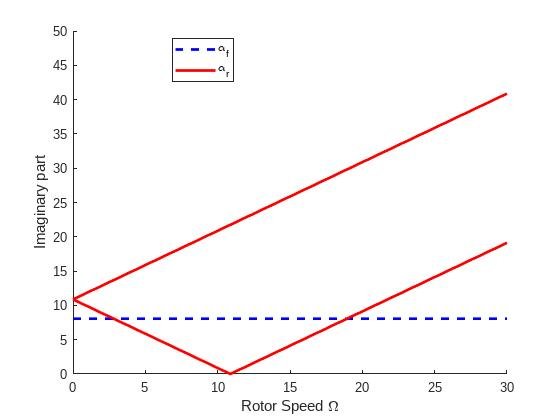
\includegraphics[width=0.7\linewidth]{gambar/Imag(uncoupled).jpg}}
	\caption{Plot grafik imajiner terhadap kecepatan rotor $\Omega$ pada kondisi sebelum dimasukkan kondisi \textit{coupled} pada sistem.}
	\label{fig:imag(uncoupled)}
\end{figure}

Pada grafik \ref{fig:imag(uncoupled)} garis putus-putus berwarna biru merupakan nilai eigen untuk \textit{fuselage} helikopter, sehingga pada bagian imajiner tersebut memberikan besarnya mode dari \textit{fuselage}. Sedangkan garis yang berwarna merah merupakan nilai eigen dari mode rotor helikopter, dimana pada grafik tersebut merepresentasikan \textit{regressive rotor mode} dan \textit{progressive rotor mode}. 

\begin{figure}[H]
	\centering
	\fbox{\includegraphics[width=0.7\linewidth]{gambar/Imag(coupled)_mark.jpg}}
	\caption{Plot grafik imajiner terhadap kecepatan rotor $\Omega$ pada kondisi setelah dimasukkan kondisi \textit{coupled} pada sistem.}
	\label{fig:imag(coupled)}
\end{figure}

\begin{figure}[H]
	\centering
	\fbox{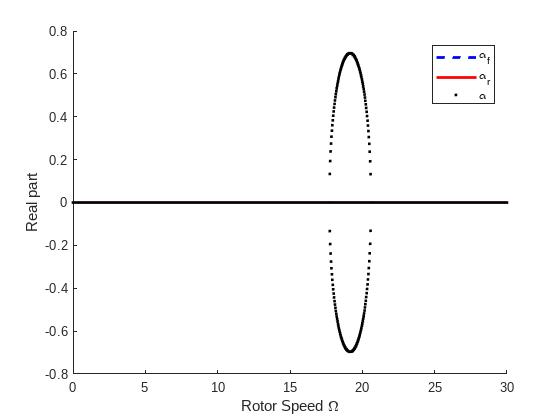
\includegraphics[width=0.7\linewidth]{gambar/Real(coupled).jpg}}
	\caption{Plot grafik riil terhadap kecepatan rotor $\Omega$ pada kondisi setelah dimasukkan kondisi \textit{coupled} pada sistem.}
	\label{fig:real(coupled)}
\end{figure}

Grafik pada gambar \ref{fig:imag(coupled)} merupakan grafik saat sistem helikopter yang memiliki interkoneksi pada bagian \textit{input} dan \textit{output} nya (\textit{coupled}). $\alpha$ merupakan nilai eigen dari sistem \textit{coupled}. Kondisi saat nilai eigen \textit{coupled} berpotongan dengan garis dari nilai eigennya pada nilai eigen di mode \textit{fuselage} nya akan mengakibatkan terjadinya \textit{ground resonance}. Gambar pada grafik \ref{fig:real(coupled)} memberikan informasi, bahwa pada bagian riil dari nilai eigen sistem \textit{coupled} berada pada nilai positif pada rentang 20.97-26.79Hz. Berdasarkan pada apa yang telah dikerjakan pada \cite{BERGEOT201672}, \cite{Eckert2007AnalyticalAA},\cite{Bergeot_passive}, dan banyak literatur mengenai fenomena \textit{ground resonance} maka pada kondisi tersebut helikopter akan mengalami getaran yang dapat menyebabkan \textit{ground resonance}. 

\begin{figure}[H]
	\centering
	\fbox{\includegraphics[width=0.65\linewidth]{gambar/find_range_10-11,89.png}}
	\caption{Plot grafik real terhadap kecepatan rotor $\Omega$ pada kondisi \textit{coupled}.}
	\label{fig:resonance_range}
\end{figure}

Gambar \ref{fig:resonance_range} merupakan langkah yang dilakukan untuk mencari respon helikopter yang terdapat pada interval 20.76-27Hz. Data respon helikopter berada pada A2 hingga A4540. Langkah ini dilakukan untuk mengonfirmasi apakah dari perhitungan matematis, helikopter memiliki potensi mengalami fenomena \textit{ground resonance} atau tidak. Namun dari hasil tersebut dapat diperhatikan bahwa memang terdapat respon yang berada pada rentang 20.76-27Hz akan tetapi dikarenakan besarnya amplitudo pada respon frekuensi tersebut tidak begitu besar, maka pada kondisi di lapangan helikopter tidak mengalami fenomena \textit{ground resonance}. Adanya batas siklus osilasi ini setidaknya memberikan informasi, bahwa pada rentang frekuensi tersebut memiliki potensi untuk mengalami fenomena \textit{ground resonance}. Disisi lain, adanya respon setelah \textit{input} yang diberikan berhenti pada helikopter pada dasarnya merupakan kompensasi dari adanya respon frekuensi yang berada pada rentang frekuensi resonansi helikopter.

\section{Potensi \textit{Ground Resonance} pada bentuk Modifikasi Penambahan Massa}

Diasumsikan bahwa pada $m_y$ terdapat penambahan massa baru sebesar $m_m$. Sehingga pada persamaan yang mengandung $m_y$ pada matriks A \ref{eq:state-space} akan menjadi $m'_y$. dengan:

\begin{align}
	\label{eq:modified}
	m'_y=m_y+m_m
\end{align}

Sehingga akan dilakukan perhitungan, saat $m_m = 0$ hingga penambahan sampai pada $m_m = 300$ yang menandakan bahwa perubahan pada massanya akan bertambah sebesar 300kg. Akan tetapi dalam perhitungan terhadap potensi fenomena \textit{ground resonance} ini memiliki batas penambahan maksimum, yaitu sebesar 4500kg. Sehingga nilai pertambahan maksimum pada modifikasi helikopter adalah sebesar 2094 kg. Selanjutnya akan coba dilihat melalui grafik seperti pada gambar grafik \ref{fig:imag(coupled)} dan \ref{fig:real(coupled)} untuk kondisi modifikasi penambahan massa pertama, yaitu sebesar 300kg. Maka akan didapatkan grafik berikut:

\begin{figure}[H]
	\centering
	\fbox{\includegraphics[width=0.65\linewidth]{gambar/imag(modified)_1.jpg}}
	\caption{Plot grafik imajiner terhadap kecepatan rotor $\Omega$ pada kondisi \textit{coupled} sebelum (hitam) dan setelah penambahan massa 300kg (hijau).}
	\label{fig:imag(modified)_1}
\end{figure}

\begin{figure}[H]
	\centering
	\fbox{\includegraphics[width=0.65\linewidth]{gambar/real(modified)_1.jpg}}
	\caption{Plot grafik riil terhadap kecepatan rotor $\Omega$ pada kondisi \textit{coupled} sebelum (hitam) dan setelah penambahan massa 300kg (hijau).}
	\label{fig:real(modified)_1}
\end{figure}

Dari kedua grafik diatas, tidak terdapat perbedaan pada bagian imajiner dan riilnya terhadap sebelum dan sesudah penambahan massa sebesar 300kg. Oleh karena itu selanjutnya akan dicoba penambahan yang lebih berat, yaitu sebesar 1000kg atau sebesar 1 ton. Sehingga akan didapatkan grafik sebagaimana berikut ini:

\begin{figure}[H]
	\centering
	\fbox{\includegraphics[width=0.65\linewidth]{gambar/imag(modified)_2.jpg}}
	\caption{Plot grafik imajiner terhadap kecepatan rotor $\Omega$ pada kondisi \textit{coupled} sebelum (hitam) dan setelah penambahan massa 1000kg (hijau).}
	\label{fig:imag(modified)_2}
\end{figure}

\begin{figure}[H]
	\centering
	\fbox{\includegraphics[width=0.65\linewidth]{gambar/real(modified)_2.jpg}}
	\caption{Plot grafik riil terhadap kecepatan rotor $\Omega$ pada kondisi \textit{coupled} sebelum (hitam) dan setelah penambahan massa 1000kg (hijau).}
	\label{fig:real(modified)_2}
\end{figure}

Pada grafik diatas, sudah mulai terdapat perbedaan rentang frekuensi resonansi pada helikopter hasil modifikasi. Untuk frekuensi resonansi pada hasil modifikasi memiliki rentang frekuensi 21.3-26.17Hz. Hal ini berarti pada penambahan 1000kg menggeser batas siklus osilasi sebesar 0.33Hz dari batas terendah dan 0.62Hz dari batas tertinggi. Kemudian selanjutnya akan dilakukan penambahan massa pada modifikasi sebesar 2000kg, dengan pertimbangan bahwa sisa 94kg lainnya merupakan seorang pilot yang bermassa dibawah 94kg. 

\begin{figure}[H]
	\centering
	\fbox{\includegraphics[width=0.65\linewidth]{gambar/imag(modified)_3.jpg}}
	\caption{Plot grafik imajiner terhadap kecepatan rotor $\Omega$ pada kondisi \textit{coupled} sebelum (hitam) dan setelah penambahan massa 2000kg (hijau).}
	\label{fig:imag(modified)_3}
\end{figure}

\begin{figure}[H]
	\centering
	\fbox{\includegraphics[width=0.65\linewidth]{gambar/real(modified)_3.jpg}}
	\caption{Plot grafik riil terhadap kecepatan rotor $\Omega$ pada kondisi \textit{coupled} sebelum (hitam) dan setelah penambahan massa 2000kg (hijau).}
	\label{fig:real(modified)_3}
\end{figure}

Dari grafik \ref{fig:real(modified)_3} menunjukkan perubahan yang cukup siginifikan untuk batas terendah dan tertinggi pada frekuensi resonansi helikopter. Untuk batas terendah yang dimiliki helikopter berkurang sebesar 0.54Hz dan dari batas tertinggi berkurang sebesar 0.99Hz. Dari hasil perhitungan potensi fenomena \textit{ground resonance} pada helikopter modifikasi justru membuat batas siklus osilasi pada helikopter menjadi semakin kecil. Seperti yang telah ditunjukkan pada grafik gambar \ref{fig:real(modified)_2} dan \ref{fig:imag(modified)_3} maka di dapatkan informasi bahwa seiring dengan pertambahan massa, rentang batas siklus osilasi pada helikopter akan semakin kecil pula. Akan tetapi asumsi penambahan massa modifikasi pada helikopter ini didasarkan pada penambahan yang merata pada setiap titik helikopter. Oleh karena itu diperlukan analisis dari aspek geometri jika penambahan massa pada helikopter melibatkan modifikasi bentuk yang tidak merata pada helikopter. Hal tersebut dikarenakan penambahan massa yang tidak merata pada helikopter akan menyebabkan pusat massa helikopter berpindah dari pusat massa awalnya. Dengan penambahan maksimal pada massa sebesar 2000kg, didapatkan batas siklus osilasinya sebesar 21.51-25.8Hz. Sehingga bila dibandingkan dengan batas siklus osilasi $f_2$ pada standar didapatkan error sebesar 7.62$\%$.

\section{Hasil Simulasi FEMAP}

Hasil simulasi pada FEMAP menggunakan beberapa kondisi pendekatan dengan keadaan sebenarnya dari helikopter. Dalam hal ini, diberikan \textit{constraint} pada beberapa titik di helikopter. Titik tersebut terletak pada bagian depan dan tengah diposisi kanan-kiri kerangka helikopter. \textit{Constraint} tersebut merepresentasikan posisi pendaratan helikopter pada darat, yaitu ban dan oleo. Dari titik yang telah ditentukan pada tabel \ref{tb:koordinat}, yaitu terletak pada ID 9, 10, 15, dan 16 atau jika dilihat menggunakan skema pada gambar \ref{fig:skema_model} terletak pada mark 1s, 1s', 3s dan 3s'. \textit{Constraint} yang diberikan merupakan batasan yang hanya berada pada arah sumbu-x. Sehingga pada titik tersebut tidak terdapat perindahan secara translasi.

Helikopter dimodelkan berdasarkan model stik atau batang. Pada masing-masing penghubung stiknya merupakan \textit{node}. Digunakan material berbahan dasar titanium untuk elemen pada stik pemodelan helikopter. Pendekatan propertis material titanium menggunakan informasi yang terdapat pada \cite{ASTM}.

\begin{figure}[H]
	\centering
	\fbox{\includegraphics[width=0.6\linewidth]{gambar/simulasi_tampak_atas.jpg}}
	\caption{Gambar hasil pemodelan stik helikopter tampak dari atas.}
	\label{fig:simulasi_tampak_atas}
\end{figure}

\begin{figure}[H]
	\centering
	\fbox{\includegraphics[width=0.6\linewidth]{gambar/simulasi_tampak_depan.jpg}}
	\caption{Gambar hasil pemodelan stik helikopter tampak dari depan.}
	\label{fig:simulasi_tampak_depan}
\end{figure}

\begin{figure}[H]
	\centering
	\fbox{\includegraphics[width=0.6\linewidth]{gambar/simulasi_tampak_samping.jpg}}
	\caption{Gambar hasil pemodelan stik helikopter tampak dari samping.}
	\label{fig:simulasi_tampak_samping}
\end{figure}

\begin{figure}[H]
	\centering
	\fbox{\includegraphics[width=0.6\linewidth]{gambar/simulasi_tampak_normal.jpg}}
	\caption{Gambar hasil pemodelan stik helikopter tampak dari normal.}
	\label{fig:simulasi_tampak_normal}
\end{figure}

Dari pemodelan yang telah dibuat pada FEMAP, selanjutnya telah digunakan analisis pada fitur FEMAP untuk mencari \textit{mode shape} pada helikopter. Secara matematis, pada dasarnya untuk mencari \textit{mode shape} pada helikopter adalah dengan mencari nilai eigen dari sistem pemodelannya. Kemudian dari nilai eigen tersebut didapatkan vektor eigen untuk selanjutnya dapat merepresentasikan gerakan dari n-mode yang dimilki oleh helikopter. Dalam hal ini telah didapatkan 10 mode pada helikopter.

Pada gambar \ref{fig:mode1} hingga \ref{fig:mode10} merupakan deformasi mode 1 hingga mode 10. Setiap mode memiliki bentuk deformasi dan frekuensi yang berbeda-beda. Mode 1 hingga 3 memiliki frekuensi yang sangat kecil, dari ketiga \textit{mode shape} tersebut memiliki gerakan yang hampir sama. Kemudian pada mode 4 hingga 10 memiliki frekuensi dan \textit{mode shape} yang berbeda-beda pula. Bila dikembalikan pada pemahaman teoritis, fenomena \textit{ground resonance} dapat terjadi apabila peredam pada bilah rotor tidak dapat mengkompensasi gerakan tertinggal bilahnya (\textit{lead/lag motion}) maka pusat massa helikopter tidak akan segaris lagi dengan rotor. Hal tersebut dapat menyebabkan ketidakstabilan oleh gaya sentrifugal pada frekuensi tertentu yang menyebabkan badan helikopter mengalami getaran dan saat frekuensi dari rotor memiliki nilai yang mendekati frekuensi natural helikopter maka terjadilah \textit{ground resonance}. Hal ini seperti yang ditunjukkan pada gambar \ref{fig:simulasiGR}.

\begin{figure}[H]
	\begin{subfigure}{0.49\textwidth}
		\centering
		\fbox{\includegraphics[width=0.9\linewidth]{gambar/mode1.jpg}}
		\caption{}
		\label{fig:mode1}
	\end{subfigure}
	\centering
	\begin{subfigure}{0.49\textwidth}
		\centering
		\fbox{\includegraphics[width=0.9\linewidth]{gambar/mode2.jpg}}
		\caption{}
		\label{fig:mode2}
	\end{subfigure}
	\caption{Deformasi pada: (a) mode 1 di frekuensi 3.55*$10^-7$Hz (b) mode 2 di frekuensi 3.56*$10^-6$Hz.}
\end{figure}

\begin{figure}[H]
	\begin{subfigure}{0.49\textwidth}
		\centering
		\fbox{\includegraphics[width=0.9\linewidth]{gambar/mode3.jpg}}
		\caption{}
		\label{fig:mode3}
	\end{subfigure}
	\centering
	\begin{subfigure}{0.49\textwidth}
		\centering
		\fbox{\includegraphics[width=0.9\linewidth]{gambar/mode4.jpg}}
		\caption{}
		\label{fig:mode4}
	\end{subfigure}
	\caption{Deformasi: (a) mode 3 pada frekuensi $3.85*10^-7$Hz (b) mode 4 pada frekuensi 2.57Hz.}
\end{figure}

\begin{figure}[H]
	\begin{subfigure}{0.49\textwidth}
		\centering
		\fbox{\includegraphics[width=0.9\linewidth]{gambar/mode5.jpg}}
		\caption{}
		\label{fig:mode5}
	\end{subfigure}
	\centering
	\begin{subfigure}{0.49\textwidth}
		\centering
		\fbox{\includegraphics[width=0.9\linewidth]{gambar/mode6.jpg}}
		\caption{}
		\label{fig:mode6}
	\end{subfigure}
	\caption{Deformasi: (a) mode 5 pada frekuensi 2.58Hz (b) mode 6 pada frekuensi 4.06Hz.}
\end{figure}

\begin{figure}[H]
	\begin{subfigure}{0.49\textwidth}
		\centering
		\fbox{\includegraphics[width=0.9\linewidth]{gambar/mode7.jpg}}
		\caption{}
		\label{fig:mode7}
	\end{subfigure}
	\centering
	\begin{subfigure}{0.49\textwidth}
		\centering
		\fbox{\includegraphics[width=0.9\linewidth]{gambar/mode8.jpg}}
		\caption{}
		\label{fig:mode8}
	\end{subfigure}
	\caption{Deformasi: (a) mode 7 pada frekuensi 5.81Hz (b) mode 8 pada frekuensi 6.88Hz.}
\end{figure}

\begin{figure}[H]
	\begin{subfigure}{0.49\textwidth}
		\centering
		\fbox{\includegraphics[width=0.9\linewidth]{gambar/mode9.jpg}}
		\caption{}
		\label{fig:mode9}
	\end{subfigure}
	\centering
	\begin{subfigure}{0.49\textwidth}
		\centering
		\fbox{\includegraphics[width=0.9\linewidth]{gambar/mode10.jpg}}
		\caption{}
		\label{fig:mode10}
	\end{subfigure}
	\caption{Deformasi: (a) mode 9 pada frekuensi 9.52Hz (b) mode 10 pada frekuensi 10.0Hz.}
\end{figure}

\begin{figure}[H]
	\centering
	\includegraphics[width=0.6\linewidth]{gambar/simulasiGR.png}
	\caption{Gaya sentrifugal dan ketidakstabilan helikopter saat \textit{ground resonance}.}
	\label{fig:simulasiGR}
\end{figure}

Dari beberapa \textit{mode shape} yang telah didapatkan, terdapat salah satu gerakan pada \textit{mode shape} yang memiliki bentuk yang serupa dengan fenomena pada gambar \ref{fig:simulasiGR}, yaitu pada mode ke-6. Pada mode tersebut, \textit{fuselage} memiliki getaran yang bergerak pada sumbu-y (kanan-kiri).

\begin{figure}[H]
	\begin{subfigure}{0.49\textwidth}
		\centering
		\fbox{\includegraphics[width=0.9\linewidth]{gambar/mode6_frame_1.PNG}}
		\caption{}
		\label{fig:mode6_frame_1}
	\end{subfigure}
	\centering
	\begin{subfigure}{0.49\textwidth}
		\centering
		\fbox{\includegraphics[width=0.9\linewidth]{gambar/mode6_frame_2.PNG}}
		\caption{}
		\label{fig:mode6_frame_2}
	\end{subfigure}
	\caption{Gerakan pada mode ke-6 saat: (a) animasi frame ke-1 (b) animasi frame ke-2.}
\end{figure}

\begin{figure}[H]
	\begin{subfigure}{0.49\textwidth}
		\centering
		\fbox{\includegraphics[width=0.9\linewidth]{gambar/mode6_frame_3.PNG}}
		\caption{}
		\label{fig:mode6_frame_3}
	\end{subfigure}
	\centering
	\begin{subfigure}{0.49\textwidth}
		\centering
		\fbox{\includegraphics[width=0.9\linewidth]{gambar/mode6_frame_4.PNG}}
		\caption{}
		\label{fig:mode6_frame_4}
	\end{subfigure}
	\caption{Gerakan pada mode ke-6 saat: (a) animasi frame ke-3 (b) animasi frame ke-4.}
\end{figure}

% Please add the following required packages to your document preamble:
% \usepackage{graphicx}
\begin{table}[h]
	\centering
	\caption{Deformasi posisi \textit{node} pada mode ke-6 berdasarkan sumbu-x, y, dan z.}
	\label{tb:deform_mode6}
	\resizebox{\textwidth}{!}{%
		\begin{tabular}{|c|c|c|c|c|c|}
			\hline
			\textbf{Results   Set ID} & \textbf{Nodes} & \textbf{Translasi total (m)} & \textbf{Translasi sumbu-x (m)} & \textbf{Translasi sumbu-y (m)} & \textbf{Translasi sumbu-z (m)} \\ \hline
			6 & 1 & 0.031166758 & 0.0041047 & -0.03088175 & -0.00091425 \\ \hline
			6 & 2 & 0.031226918 & 0.00410521 & -0.03094131 & -0.00095025 \\ \hline
			6 & 3 & 0.010508383 & 0.00194159 & -0.01027656 & -0.00102403 \\ \hline
			6 & 4 & 0.030034335 & -0.02786271 & -0.01121261 & -9.0664E-05 \\ \hline
			6 & 5 & 0.093941227 & -0.09145697 & 0.02139585 & 0.00167185 \\ \hline
			6 & 6 & 0.014890737 & -0.00358556 & 0.01442101 & -0.00095518 \\ \hline
			6 & 7 & 0.015888741 & 0.01209325 & 0.01029411 & 0.00048645 \\ \hline
			6 & 8 & 0.015742892 & 0.0118489 & 0.01035368 & 0.00049345 \\ \hline
			6 & 9 & 0.031194627 & 0 & 0.03116187 & 0.00142914 \\ \hline
			6 & 10 & 0.031447977 & 0 & 0.03141167 & 0.00151069 \\ \hline
			6 & 11 & 0.016951818 & 0.01189636 & -0.01207376 & -0.00025508 \\ \hline
			6 & 12 & 0.017044749 & 0.01207032 & -0.01203184 & -0.00025618 \\ \hline
			6 & 13 & 0.026711104 & -0.00049977 & 0.02667112 & 0.00137277 \\ \hline
			6 & 14 & 0.026702074 & -0.00040783 & 0.02667187 & 0.00120235 \\ \hline
			6 & 15 & 0.013104029 & 0 & 0.01309668 & 0.00043871 \\ \hline
			6 & 16 & 0.012999032 & 0 & 0.0129918 & 0.00043346 \\ \hline
			6 & 17 & 0.004834764 & -6.1188E-05 & -0.00477169 & -0.00077599 \\ \hline
			6 & 18 & 0.004876604 & -4.0964E-05 & -0.00481559 & -0.0007679 \\ \hline
			6 & 19 & 0.023838466 & 0.00590968 & 0.02308512 & 0.0006523 \\ \hline
			6 & 20 & 0.023781126 & 0.00619057 & 0.02295198 & 0.0006521 \\ \hline
			6 & 21 & 0.023747081 & 0.00697248 & 0.0226476 & 0.00154746 \\ \hline
			6 & 22 & 0.02347669 & 0.00732844 & 0.02230146 & -0.00030622 \\ \hline
			6 & 23 & 0.015334978 & 0.00710014 & 0.0134533 & 0.00193862 \\ \hline
			6 & 24 & 0.033077482 & 0.0044104 & -0.03276836 & -0.00095028 \\ \hline
			6 & 25 & 0.031602003 & 0.00409287 & -0.03132143 & -0.00095028 \\ \hline
			6 & 26 & 0.008696403 & 0.00727985 & -0.0047458 & -0.00032958 \\ \hline
			6 & 27 & 0.016638447 & 0.01218675 & 0.01131974 & 0.00042928 \\ \hline
			6 & 28 & 0.016724696 & 0.01256482 & 0.01102233 & 0.00059078 \\ \hline
			6 & 29 & 0.014414827 & 0.01223738 & -0.0075899 & -0.00065363 \\ \hline
			6 & 30 & 0.014725202 & 0.0125541 & -0.00768942 & 0.00031434 \\ \hline
			6 & 31 & 0.015152109 & 0.00745834 & 0.01316307 & -0.00083249 \\ \hline
			6 & 32 & 0.008928208 & 0.00751982 & -0.00480135 & -0.0003351 \\ \hline
		\end{tabular}%
	}
\end{table}

Hasil simulasi yang ditunjukkan pada mode ke-6. Berkorelasi dengan frekuensi respon pada helikopter yang didapatkan menggunakan sensor akselerometer. Untuk rentang 4 hingga 4.1Hz (dimana frekuensi mode ke-6 berada, yaitu 4.06Hz) terdapat sebanyak 16 frekuensi respon terdeteksi pada helikopter, yaitu hanya 0.66$\%$ dari total frekuensi yang berada pada rentang 0 hingga 80Hz. Hal ini memvalidasi, bahwa apabila ditinjau dari \textit{finite element analysis} menggunakan FEMAP, tidak terdapat potensi yang besar untuk terjadinya fenomena \textit{ground resonance} pada helikopter hasil modifikasi ini. Apabila ditinjau secara kuantitatif, perpindahan secara translasi pada masing-masing \textit{node} di helikopter ditampilkan pada tabel \ref{tb:deform_mode6}. Tabel tersebut didapatkan secara komputasi pada \textit{software} FEMAP. Adapun tabel deformasi pada mode yang lainnya akan ditampilkan pada lampiran.